\documentclass{mythesis}
\usepackage{mythesis}

%% You can set the line spacing this way
%\setallspacing{double}
%% or a section at a time like this
%\setfrontmatterspacing{double}

%% PDF metadata
\makeatletter
\@ifpackageloaded{hyperref}{%
\hypersetup{%
pdftitle = {Studying B to K pi decays with LHCb},
pdfsubject = {Andy Buckley's PhD thesis},
pdfkeywords = {LHCb, B, physics, LHC, heavy flavour},
pdfauthor = {\textcopyright\ Andy Buckley}
}
}{}
\makeatother

%% Define the thesis title and author
\title{Measuring the Polarisation of the \PW boson and Searching for
  Supersymmetry at CMS} \author{Alexander Sparrow}

%% Start the document
\begin{document}

\begin{acronym}
\acro{NP}{New Physics}
\acro{SM}{Standard Model}
\acro{ALICE}{A Large Ion Collider Experiment}
\acro{ATLAS}{A Toroidal LHC Apparatus}
\acro{LHCb}{Large Hadron Collider Beauty Experiment}
\acro{TOTEM}{Total Elastic and diffractive cross section Measurement}
\acro{LHCf}{Large Hadron Collider Forward}
\acro{CMS}{Compact Muon Solenoid}
\acro{LHC}{Large Hadron Collider}
\acro{CERN}{Conseil Européen pour la Recherche Nucléaire}
\acro{LEP}{Large Electron-Positron Collider}
\acro{PSB}{Proton Synchrotron Booster}
\acro{PS}{Proton Synchrotron}
\acro{SPS}{Super Proton Synchrotron}
\acro{LEIR}{Low Energy Ion Storage Ring}
\acro{ECAL}{Electromagnetic Calorimeter}
\acro{EB}{ECAL Barrel}
\acro{EE}{ECAL Endcap}
\acro{TIB}{Tracker Inner Barrel}
\acro{TOB}{Tracker Outer Barrel}
\acro{TID}{Tracker Inner Disk}
\acro{TEC}{Tracker Endcap}
\acro{APD}{Avalance Photodiode}
\end{acronym}

%% Define the un-numbered front matter (cover pages, rubrik and table of contents)
\begin{frontmatter}
  %% Title
\titlepage[of Imperial College London]%
{A dissertation submitted to Imperial College London\\
 for the degree of Doctor of Philosophy}

\input{status.tex}

%% Abstract
\begin{abstract}%[\smaller \thetitle\\ \vspace*{1cm} \smaller {\theauthor}]
  %\thispagestyle{empty}
  Abstract to go here
\end{abstract}


%% Declaration
\begin{declaration}
  This dissertation is the result of my own work, except where explicit
  reference is made to the work of others, and has not been submitted
  for another qualification to this or any other university. This
  dissertation does not exceed the word limit for the respective Degree
  Committee.
  \vspace*{1cm}
  \begin{flushright}
    Andy Buckley
  \end{flushright}
\end{declaration}


%% Acknowledgements
\begin{acknowledgements}
  Of the many people who deserve thanks, some are particularly prominent,
  such as my supervisor\dots
\end{acknowledgements}


%% Preface
\begin{preface}
  This thesis describes my research on various aspects of the \LHCb
  particle physics program, centred around the \LHCb detector and \LHC
  accelerator at \CERN in Geneva. Waaay!

  \noindent
  % for this example, I'll just mention \ChapterRef{chap:SomeStuff}
  % and \ChapterRef{chap:MoreStuff}.
\end{preface}

%% ToC
\tableofcontents

%% Strictly optional!
\frontquote%
  {Time is a companion that goes with us on a journey. It reminds us to cherish each moment, because it will never come again. What we leave behind is not as important as how we have lived.}%
  {Jean-Luc Picard, 2371, after the destruction of the Enterprise-D}

\end{frontmatter}
%% Start the content body of the thesis
\begin{mainmatter}
  \linenumbers
  %% Actually, more semantic chapter filenames are better, like "chap-bgtheory.tex"
  \import{1-theory/}{theory}
  \import{2-expt/}{expt}
  \import{3-wpol/}{wpol}
  \import{4-susy/}{susy}
  \import{5-interpretation/}{interpretation}

  %% To ignore a specific chapter while working on another,
  %% making the build faster, comment it out like this:
  %\input{chap4}
  \nolinenumbers
\end{mainmatter}

%% AS: Added to make scons seen these files (it doesn't parse the import
%% statements above!)
\begin{comment}
  
\chapter{The Standard Model}
\section{Introduction}
It has been written before that the \acl{SM} of particle physics is perhaps the
most thoroughly tested theory of nature ever constructed. Despite decades of
experimental effort, there is not yet a single confirmed, experimental result
found to contradict the theory. In this chapter

  \chapter{The CMS Experiment at the Large Hadron Collider}
\section{Introduction}
The Large Hadron Collider (LHC) is a proton-proton ($\Pp\Pp$) accelerator
located at the CERN particle physics laboratory near Geneva, Switzerland. The
LHC is built in the tunnels formerly occupied by the LEP experiment, a
\unit{27}{\kilo\metre} long ring lying on the border between France and Switzerland. Two
beams of protons run in opposite directions around the ring and are made to
collide at four interaction points.

There are four primary experiments at the LHC: \ac{ALICE}, \ac{ATLAS}, \ac{CMS}
and \ac{LHCb}. Each one is constructed around one of the four interaction points
and records the shower of particles produced from the colliding protons. ATLAS
and CMS are large, general purpose detectors designed to search for a variety of
\ac{NP} signatures as well as making higher precision measurements of \ac{SM}
parameters. \ac{ALICE} is designed to examine the products of heavy-ion
collisions (lead-lead) in order to explore the quark gluon plasma and related
physics. Finally, the \ac{LHCb} experiment is optimised for the study of B-meson
decays. These are important for the study of CP violation within the \ac{SM} but
might also provide potential avenues for the discovery of \ac{NP}.

In addition to the four larger detectors, two smaller experiments, \ac{LHCf} and
\ac{TOTEM} lie upstream of the \ac{ATLAS} and \ac{CMS} collision points in order
to probe more specialised forward physics phenomena.

\section{The \acl{LHC}}
The \ac{LHC} is a circular $\Pp\Pp$ synchrotron with a circumference of
\unit{27}{km}. It sits in a tunnel initially constructed for the \ac{LEP}
accelerator buried at a depth of between 50 and \unit{175}{\metre} beneath the
Franco-Swiss border. At full design specifications, 2808 bunches of protons will
circulate around each direction of the ring, colliding at a centre of mass
energy of \unit{14}{\TeV}. With a proton bunch spacing of
\unit{25}{\ns}, the \ac{LHC} will eventually achieve a luminosity of
\unit{$10^{34}$}{\rpsquare{\centi\metre}\usk\reciprocal\second}.

\subsection{Accelerator Complex}
The \ac{LHC} ring itself is the final stage in an injector chain utilising a
series of accelerators built at CERN over the last 50 years. Each stage supplies
an incremental increase in the proton (or heavy ion) bunch energy. The first
stage in this chain is a linear accelerator, either the Linac2 for proton
injection or Linac3 during heavy-ion runs. The Linac2 injects protons into the
\ac{PSB} at an energy of \unit{50}{\mega\electronvolt}. Similarly, the ions
proceed first from the Linac3 to the \ac{LEIR} before finally arriving at the
\ac{PS}. From here on, the paths of the protons and heavy-ions are the
same. Proton bunches pass from the \ac{PSB} to the \ac{PS} at an energy of
\unit{1.4}{\giga\electronvolt} and then on to the \ac{SPS} at an energy of
\unit{28}{\giga\electronvolt}. Protons then arrive at the \ac{SPS}, where they
circulate around a ring \unit{2}{\kilo\metre} in diameter, and increasing their
energy to \unit{450}{\giga\electronvolt}. From here, kicker magnets inject the
bunches into the \ac{LHC} itself, where the energy is finally increased to the
design specified \unit{7}{\TeV} per beam.
\begin{figure}
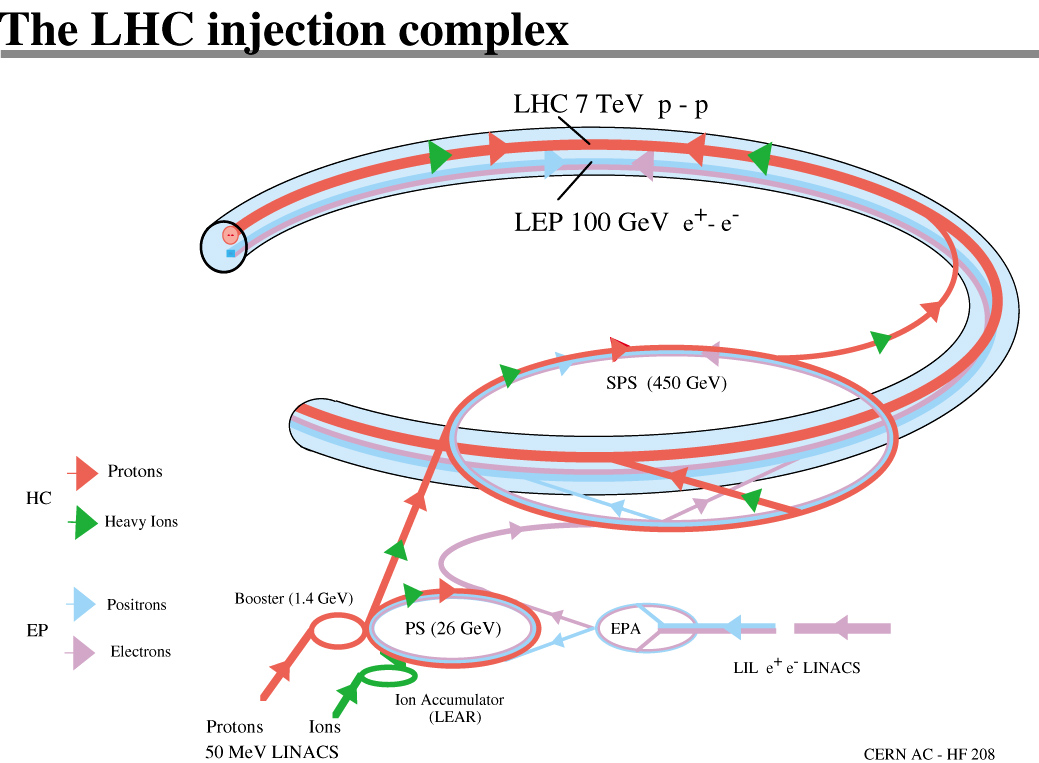
\includegraphics[width=0.9\textwidth]{fig/lhc-pho-1993-008}
\end{figure}

\ctable[
cap=LHC Accelerator Complex,
caption=LHC Accelerator Complex,
mincapwidth=0.5\textwidth,
pos=h
]{lcc}{
\tnote[a]{Heavy-Ions only}
}{\FL
Accelerator & Energy \ML
%
Linac2   & \unit{50}{\mega\electronvolt} \NN
Linac3\tmark[a]   & \unit{4.2}{\mega\electronvolt\per u} \ML
%
\acf{PSB} & \unit{1.4}{\giga\electronvolt} \NN
\acf{LEIR}\tmark[a]   & \unit{??}{\mega\electronvolt\per u} \ML
%
\acf{PS} & \unit{28}{\giga\electronvolt} \NN
\acf{SPS} & \unit{450}{\giga\electronvolt} \NN
\acf{LHC} & \unit{7}{\tera\electronvolt} \LL
}


\section{The \acl{CMS} Experiment}
\ac{CMS} is a large, general purpose detector designed to firmly establish or
disprove the existence of the Higgs boson particle as well as performing
searches for a wide variety of \ac{NP} signatures. The design goals of CMS were
as follows (paraphrasing Design proposal):
\begin{enumerate}
\item a high quality, redundant muon system,
\item the best possible \ac{ECAL}
\item high quality central tracking to complement these two systems
\item an affordable detector
\end{enumerate}

These goals motivated the design of a traditional cylindrical detector,
\unit{21.5}{\metre} in length and \unit{15}{\metre} in diameter. A key feature
of the design is the \unit{4}{\tesla} superconducting solenoid. The bending
field supplied provides accurate muon momentum resolution up to energies of
\unit{$\approx$ 1}{\TeV}. The size of the solenoid placed stringent
limitations on the volume of the inner detector subsystems (everything except
for the muon chambers and return yoke).

\subsection{Coordinate System}
In order to facilitate discussion of the detector, a right-handed coordinate
system is defined with the origin chosen to be the nominal collision point
inside \ac{CMS}. The $x$ axis is then defined to point horizontally inwards
towards the centre of the \ac{LHC} ring and the $y$-axis vertically
upwards. Therefore the $z$-axis is aligned along the beamline pointing towards
the nearby Jura mountains. Often a cylindrical coordinate system will be used
with where the azimuthal angle $\phi$ and radial coordinate $r$ span the $x-y$
plane. The azimuthal angle is measured with respect to the $x$-axis. The
pseudorapidity, $\eta = - \ln \tan \frac{\theta}{2}$ where $\theta$ is the polar
angle measured with respect to the $z$-axis.

\subsection{Silicon Tracker}
The innermost subsystem of \ac{CMS} is the silicon tracker, designed to provide
highly precise measurements of particle trajectories close to the CMS
interaction point. The tracker extends to pseudorapidities of $|\eta|<2.5$ and
has an active silicon area of more than \unit{200}{\metre\squared} making it the
largest silicon tracker ever built.

The tracker design can be better understood by considering the expected particle
flux at design luminosity as a function of radial distance $r$ from the
beamline.

\begin{itemize}
\item At $ r \approx \unit{10}{\cm}$ the particle flux is highest. Accordingly,
  the innermost layer of the CMS tracker is comprised of hybrid pixels. With an
  area of \unit{$100\times 150$}{\micro\metre\squared}, particle densities are
  $O(10^{-4})$ per pixel per LHC bunch crossing.
\item At a radius \unit{$20 < r < 55$}{\centi\metre}, reduced particle flux allows
  the use of silicon microstrip sensors. With a much larger area of
  $\unit{10}{\centi\metre}\times\unit{80}{\micro\metre}$, average particle
  densities are $O(10^{-2})$ per strip per bunch crossing.
 \item At $ r > \unit{55}{\cm}$, the silicon strip size is once again increased
   to $\unit{25}{\cm}\times \unit{180}{\cm}$ again giving a particle density of
   $O(10^{-2})$ per strip per bunch crossing.
\end{itemize}

\subsubsection{Pixel Tracker}
The hybrid pixels are placed closest to the interaction point. As well as
maintaining an acceptable particle density per sensor, their close proximity to
the interaction point allows the origin of collision products to be accurately
determined. This is of particular importance for instance in B-tagging. In the
barrel region, 3 layers are placed at mean radii of 4.4, 7.3 and
\unit{10.2}{\cm}. The detector has a length of \unit{53}{\cm} in the $z$
direction. The end discs are instrumented with only two layers and are located
at $|z|=34.5, \unit{46.5}{\cm}$. The pixel modules in these layers are arranged
in a turbine-like layout.

To acheive the desired spatial resolution, the pixels have an almost square
geometry with an area of \unit{$150\times 100$}{\micro\metre\squared} in the
$r\phi\times z$ ($r\times r\phi$) for the barrel (end discs).

\subsubsection{Strip Tracker}
Further from the interaction point, the tracker is instrumented with silicon
strip detectors. The barrel component can be further divided into the \ac{TIB}
and the \ac{TOB}. The \ac{TIB} is composed of 4 layers with the \ac{TOB}
comprising a further 6. The \ac{TOB} extends to $z = \pm
\unit{118}{\centi\metre}$. Beyond this are the endcaps which can again be split
into two components: the \ac{TEC} made up of 9 disks and the \ac{TID} 3. The
silicon micro strip sensors are \unit{320}{\micro\metre} thick and oriented
parallel to the $z$ axis in the barrel and radially in the disks.

Both the \ac{TIB} and \ac{TID} supply up to four measurements of $r\phi$. With a
strip-pitch of \unit{80}{\micro\metre} in the inner two layers and
\unit{120}{\micro\metre} in the outer two, the \ac{TIB} achieves a single point
resolution of \unit{23 and 35}{\micro\metre} respectively. In the \ac{TID}, the
strip pitch varies between \unit{100 and 141}{\micro\metre}.

The \ac{TOB} uses \unit{500}{\micro\metre} thick sensors with a strip-pitch of
\unit{183}{\micro\metre} in the first four layers and \unit{122}{\micro\metre} in
the outer two. This gives a single point resolution of \unit{53}{\micro\metre}
and \unit{35}{\micro\metre} respectively.

The first two layers of the \ac{TIB}, \ac{TOB} and \ac{TID} and rings 1, 2 and 5
of the \ac{TEC} are so-called stereo modules. These are double-sided modules
where the two layers of strips have a stereo angle of \unit{100}{\milli\radian}
between them. This provides additional resolution in the $z$ measurement in the
barrel (or $r$ in the endcaps). The resolution of this measurement is
\unit{230}{\micro\metre} and \unit{530}{\micro\metre} in the \ac{TIB} and
\ac{TOB} respectively.

\begin{figure}
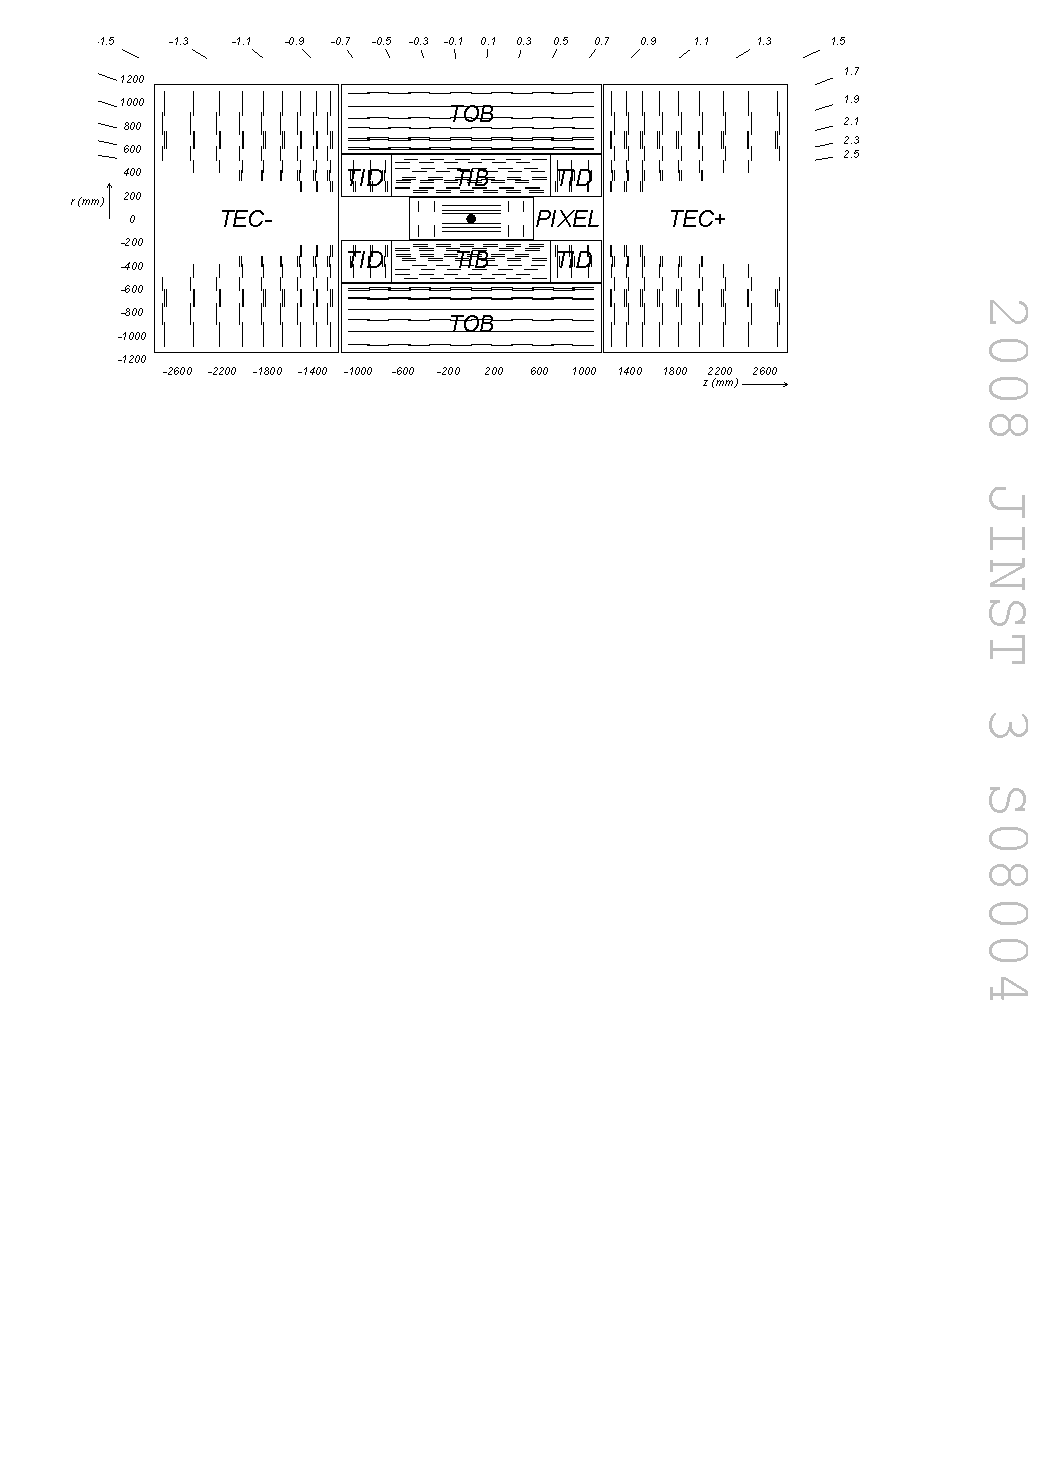
\includegraphics[width=\textwidth]{fig/tracker}
\end{figure}

\subsection{\acl{ECAL}}
The \ac{ECAL} surrounds the silicon tracker and provides a high resolution
measurement of electromagnetic showers within a homogeneous, hermetic
calorimeter composed of 61,200 lead tungstate (PbWO$_4$) crystals. This material
was chosen for its high desnity, short radiation length and small Moli\`{e}re
radius. Scintillation photons are then recorded by \ac{APD}s in the barrel and
\ac{VPT}s in the endcap. The driving motivation for the \ac{ECAL} design was the
detection of the low-mass favoured Higgs decay channel
$PH\longrightarrow\gamma\gamma$.

\subsubsection{\acl{EB}}
The \ac{EB} extends in rapidity to $|\eta|<1.479|$ with a crystal
segmentation of $360\times 85$ ($\eta-\phi$) in each half barrel. Each crystal
is slightly tapered with a cross-section of $0.0174\times0.0174$ in
$\eta-phi$. The crystals have a front cross section of \unit{$22\times
  22$}{\milli\metre\squared} and a length of \unit{230}{\milli\metre}
(corresponding to 25.8 radiation lengths).

\subsubsection{\acl{EE}}
The \ac{EE} occupies the rapidity range $1.479 < |\eta| < 3.0$. Crystals are
grouped into $5\times 5$ supercrystals within a carbon-fibre alveolar
structure. The endcaps are split into two halves, known as Dees, each holding
3,662 crystals.

The scintillation of the ac{ECAL} crystals as well as the amplification of the
\ac{APDs} varies as a function of temperature. This variation was found to be
\unit{$\approx 4\%$}{\per\celsius}. For this reason, the \ac{ECAL} temperature
is precisely regulated to within \unit{$\pm$ 0.05}{\celsius}.

\subsection{\acl{HCAL}}
Accurate measurement of hadronic showers is crucial for analyses involving jets
or missing energy type signatures. The \ac{HCAL} lies between the outer edge of
the ECAL and the inner edge of the solenoid ($\unit{1.77}{\metre} < r <
\unit{2.95}{\metre}$). This constrains the size of the \ac{HCAL} to a relatively
compact design and necessitates the placement of a ``tail catcher'' outside of
the solenoid.

\subsubsection{\acl{HB}}
\subsubsection{\acl{HE}}


\subsection{Magnet}
\subsection{Muon Chambers}
As has already been said, sensitive detection of muons is one of \ac{CMS}'s key
design goals. Since the effect of radiative losses in the tracker is much less
for muons than it is for electrons, muons are able to provide a much finer mass
resolution which can be used in a variety of physics searches and
measurements. The muon system at CMS is responsible for muon identification,
momentum measurement and triggering (for further detail see
Section~\ref{sec:trigger}). Three types of detectors are used, chosen for
different regions of the detector according to the magnetic field, muon rate and
response time required for input to the trigger.

\subsubsection{\acl{DT}}
In the barrel region, the magnetic field is relatively uniform and the muon flux
low enough to allow the use of drift tubes. These identify muons in the region
$|\eta| < 1.2$. The drift chamber was first developed as a refinement of earlier
wire proportional chamber designs in which the drift time of the electrons to
the anode wire is used to provide additional spatial resolution. This allows the
wire spacing to be increased thus reducing the electronics requirements.

Each drift chamber is composed of 2 (or 3) superlayers, which are further
divided into 4 layers of rectangular drift cells. Of the four concentric muon
stations in the barrel, the inner three contains 60 drift chambers and the
outermost 70. The wires in the outer two layers of each drift cell are oriented
parallel to the beam line, providing a measurement in the $r\phi$ direction (the
magnetic bending plane). The inner two layers are perpendicularly aligned,
giving a measurement of the $z$ coordinate.

\subsubsection{\acl{CSC}}
In the endcap region, the large muon and background rate coupled with the large,
non-uniform magnetic field prevent the use of \ac{DT}s. Instead, \acl{CSC}s are
used. The CMS Muon endcap consists of 468 \ac{CSC}s, each a trapezoidal
multiwire proportional chamber arranged radially covering an azimuthal angle
$\Delta\phi$ of either 10 or 20 degrees. Each \ac{CSC} is a multiwire
proportional chamber with 6 anode wire planes interleaved with 7 cathode strip
planes. The wire readout provides a measurement of the $\phi$ coordinate whilst
$r$ position information is obtained by interpolating charges on the cathode
strips.

\subsubsection{\acl{RPC}}
In order to provide a fast trigger signal (see Section~\ref{sec:trigger}), a
muon detector capable of providing a fast signal is required. This is the
\acl{RPC}, a gaseous parallel-plate detector with spatial resolution suitable
for both barrel and endcap regions and a response time much less than the
\unit{25}{\nano\second} between consecutive \ac{LHC} bunch crossings.

\subsection{Data Aquisition and Trigger System}
The high luminosity at the \ac{LHC} brings with it a large particle flux. Along
with the requirements of precise position and momentum measurements, this has
motivated the fine granularity present across each \ac{CMS} subdetector. The
natural consequence of this is an extremely large number of readout channels,
approximately \unit{55}{\million} across the whole detector. To make matters
worse, it is planned that the \ac{LHC} will eventually reach a bunch spacing of
only \unit{25}{\nano\second}. This places a tight latency requirement on the
\ac{DAQ} system.

Tightly coupled to the \ac{DAQ} is the trigger system. The huge number of
readout channels in \ac{CMS} is not only a problem in terms of the bandwidth of
the \ac{DAQ} but also poses serious problems relating to long-term storage
requirements. A digited, zero-supressed event dump from \ac{CMS} is
approximately \unit{2}{\mega\byte} in size. With an event rate of upto
\unit{40}{\mega\hertz}, this would potentially require a storage rate of
\unit{80}{\tera\byte\per\second}. Even with the rapid improvement of disk
storage technology over the last few decades, such storage capacities are
clearly infeasible both in terms of capacity and \ac{IO} requirements. For these
reasons, a system capable of quickly rejecting a very large fraction of
collisions is required. This is known as the trigger.

  \chapter{Measuring the Helicity Polarisation of the $\PW$ Boson}
\section{Introduction}
The study of \Wjets production at a hadron collider presents an important
opportunity for furthering understanding of the underlying Electroweak and
\ac{QCD} processes. In particular, since it is one of a relatively small number
of processes for which highly precise \ac{NLO} calculations have been performed,
experimental measurements can give a direct constraint on the \acp{PDF}. \Wjets
production is also of considerable interest in the context of \ac{NP} searches
where these events are often a dominant background. Finally, the neutrino in the
leptonic decay mode provides a source of ``real'' missing energy which can be
useful in the understanding of detector effects relevant to searches for
\acs{WIMP}-type particles present in \ac{SUSY} and other theories.

\section{Background}
Some theoretical background relating to \PW helicity effects has been presented
in Section~TODO. Here, the discussion will be oriented towards a more
experimental context.

For small values of \PW transverse momentum, \PtW the differential angular
cross-section for the process
$\Pp\Pp\longrightarrow\PWpm\longrightarrow\Plpm\Pgnl$ follows the Drell-Yan
distribution
\begin{equation}
\frac{dN}{d(\cos\theta)} \propto (1\mp \cos\theta)^2
\end{equation}

It is well known from straightforward helicity arguments\cite{mirkes_w_1994}that
\PW produced along the beam axis will exhibit a 100\% left-handed polarization. This
can be seen by considering the leading order partonic subprocesses
\begin{equation}
\Pup\APdown \longrightarrow \PWp \qquad\textrm{and}\qquad
\Pdown\APup\longrightarrow\PWm
\end{equation}
Firstly, note that the fraction of the proton momentum carried by the quark (as
determined by the \aclp{PDF}) is greater than that of the anti-quark. In
addition given that the \ac{LHC} is a $\Pp\Pp$ collider, valence anti-quarks are
not present. Anti-quarks must be drawn from the sea and are therefore likely to
be low momentum. Taking these two facts together, the quark is very likely to be
higher momentum than the anti-quark. By momentum conservation, it is expected
that the \PW will be produced overwhelmingly in the direction of the original
quark. Then given the \VminusA nature of the weak interaction, it is seen that
the quark must be left-handed and, by helicity conservation the \PW will be
polarised nearly 100\% left-handedly along the beam axis. A small dilution will
occur in instances where the anti-quark has by chance a larger momentum fraction
than the quark.

It is worth mentioning that the situation is not identical at the Tevatron
$\Pp\Pap$ collider. Although the \PWp also possess a 100\% left-handed
polarisation along the beamline (via similar arguments to those given above),
the \PWm are found to have a near 100\% right-handed polarisation. This is a
result of the subprocess $\APup\Pdown\longrightarrow\PWm$ where this time the
\APup carries more momentum.

In the case, where the \PW carries a significant transverse momentum \PtW, the
situation is more complex.


\begin{figure}
\centering
\subfloat[]{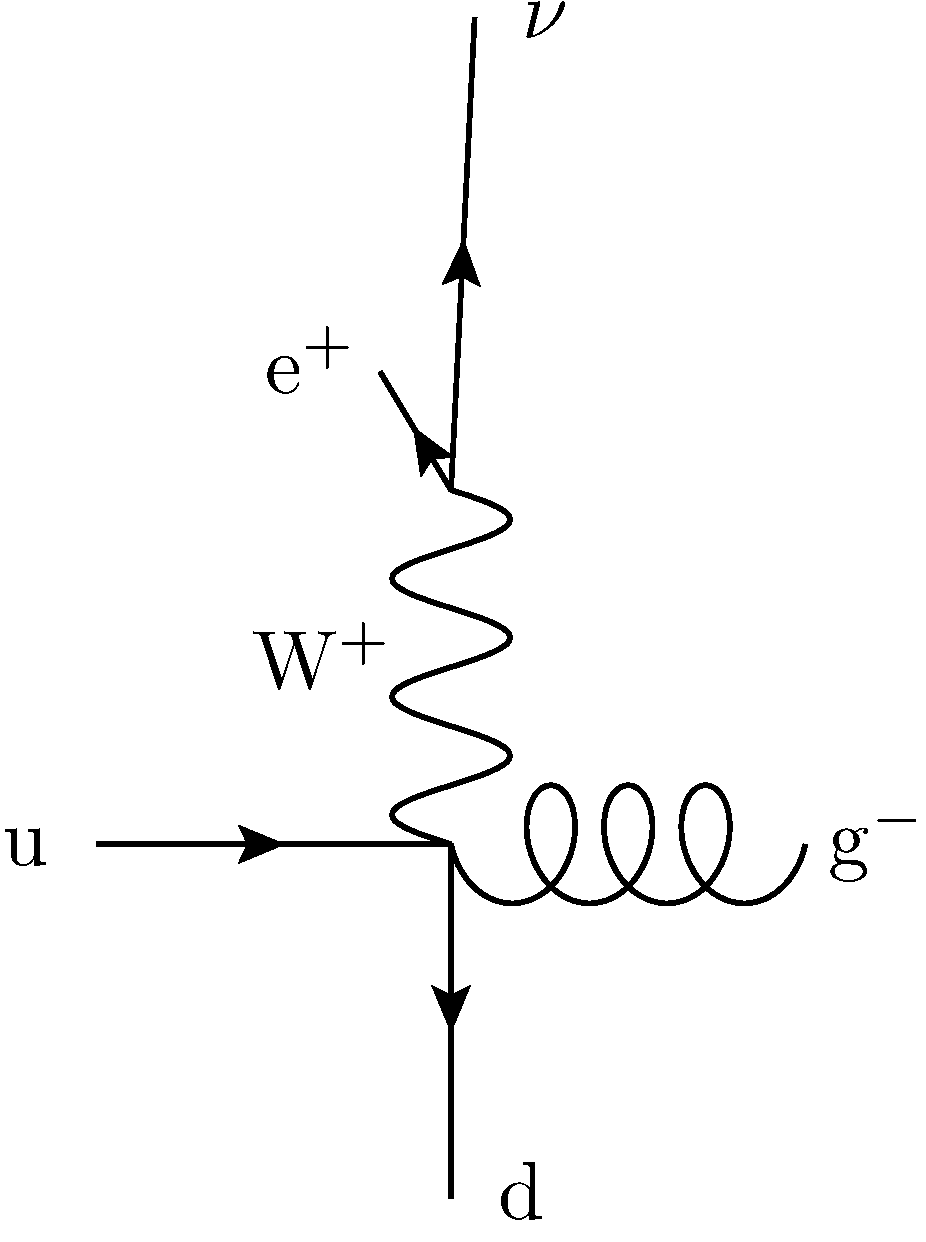
\includegraphics[width=0.3\textwidth]{fig/wpol_prod_a}}\quad
\subfloat[]{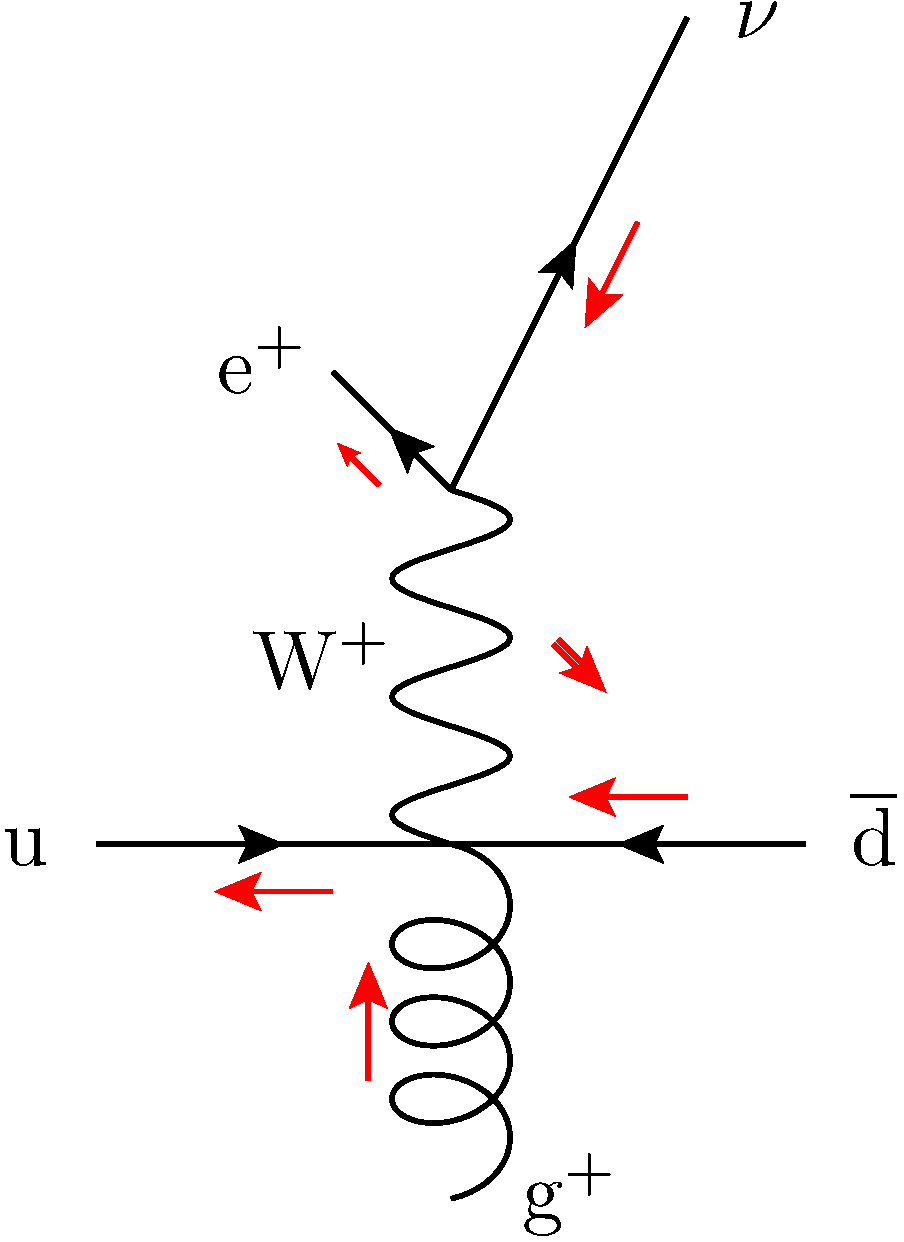
\includegraphics[width=0.3\textwidth]{fig/wpol_prod_b}}\quad
\subfloat[]{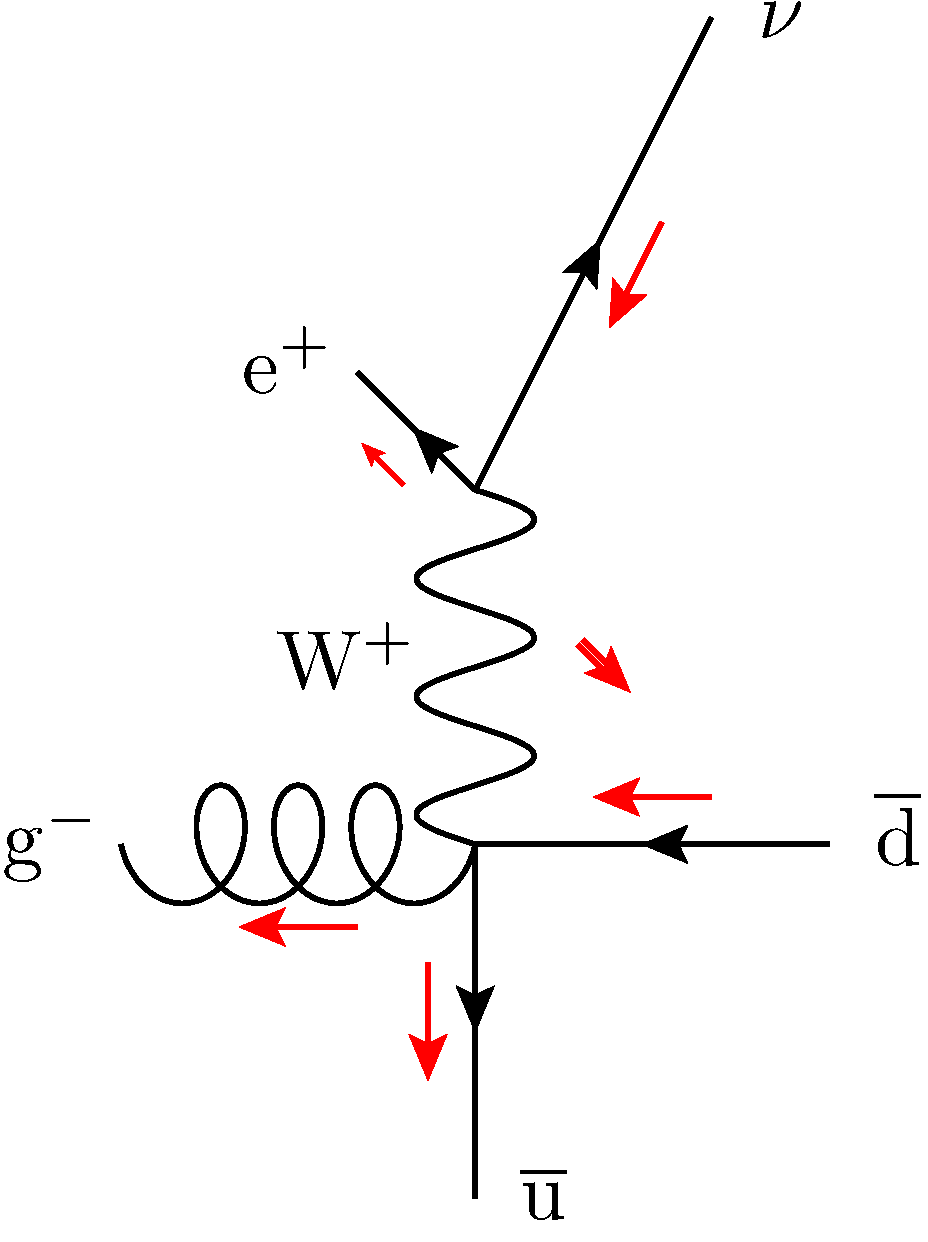
\includegraphics[width=0.3\textwidth]{fig/wpol_prod_c}}\\
\subfloat[]{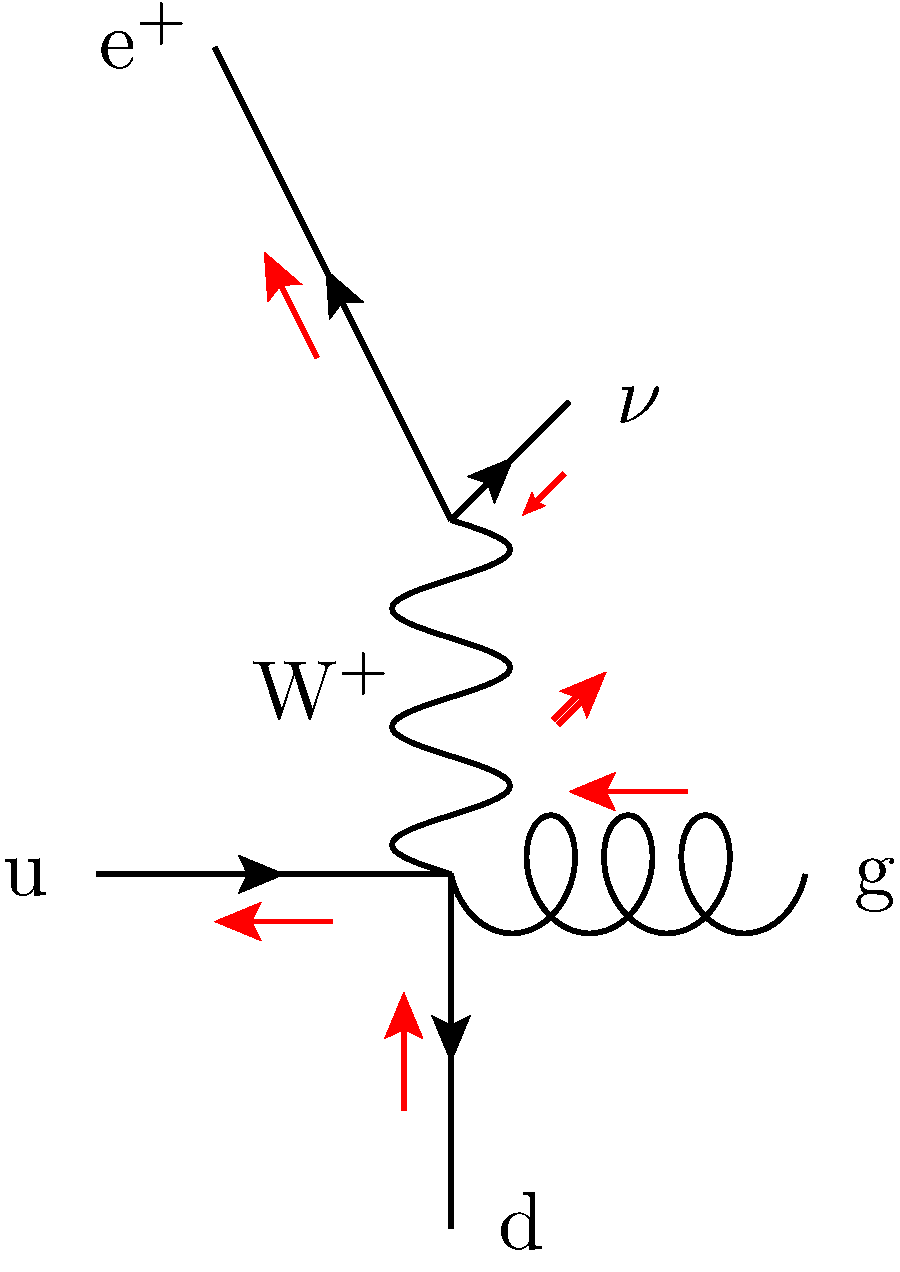
\includegraphics[width=0.3\textwidth]{fig/wpol_prod_d}}\quad
\subfloat[]{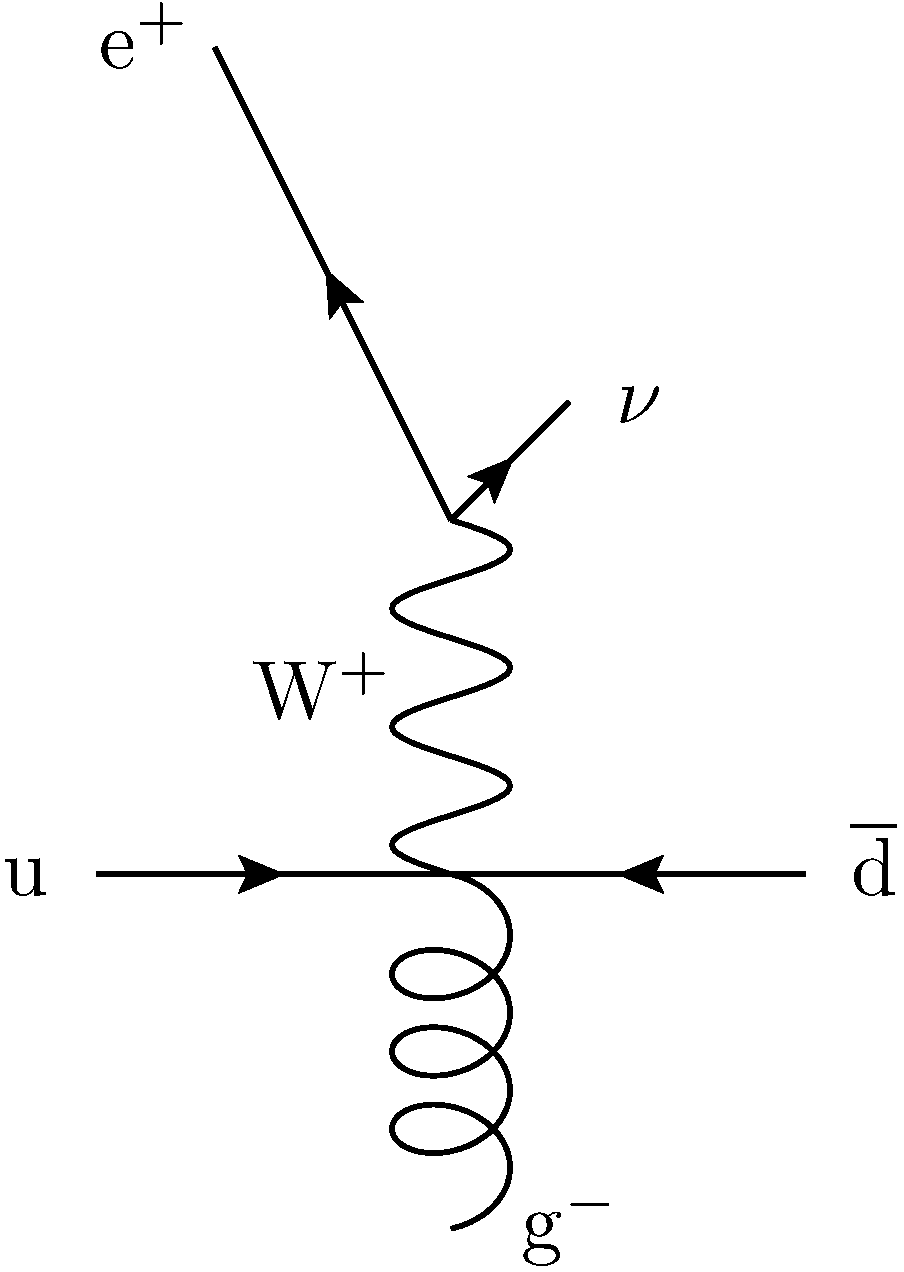
\includegraphics[width=0.3\textwidth]{fig/wpol_prod_e}}\quad
\subfloat[]{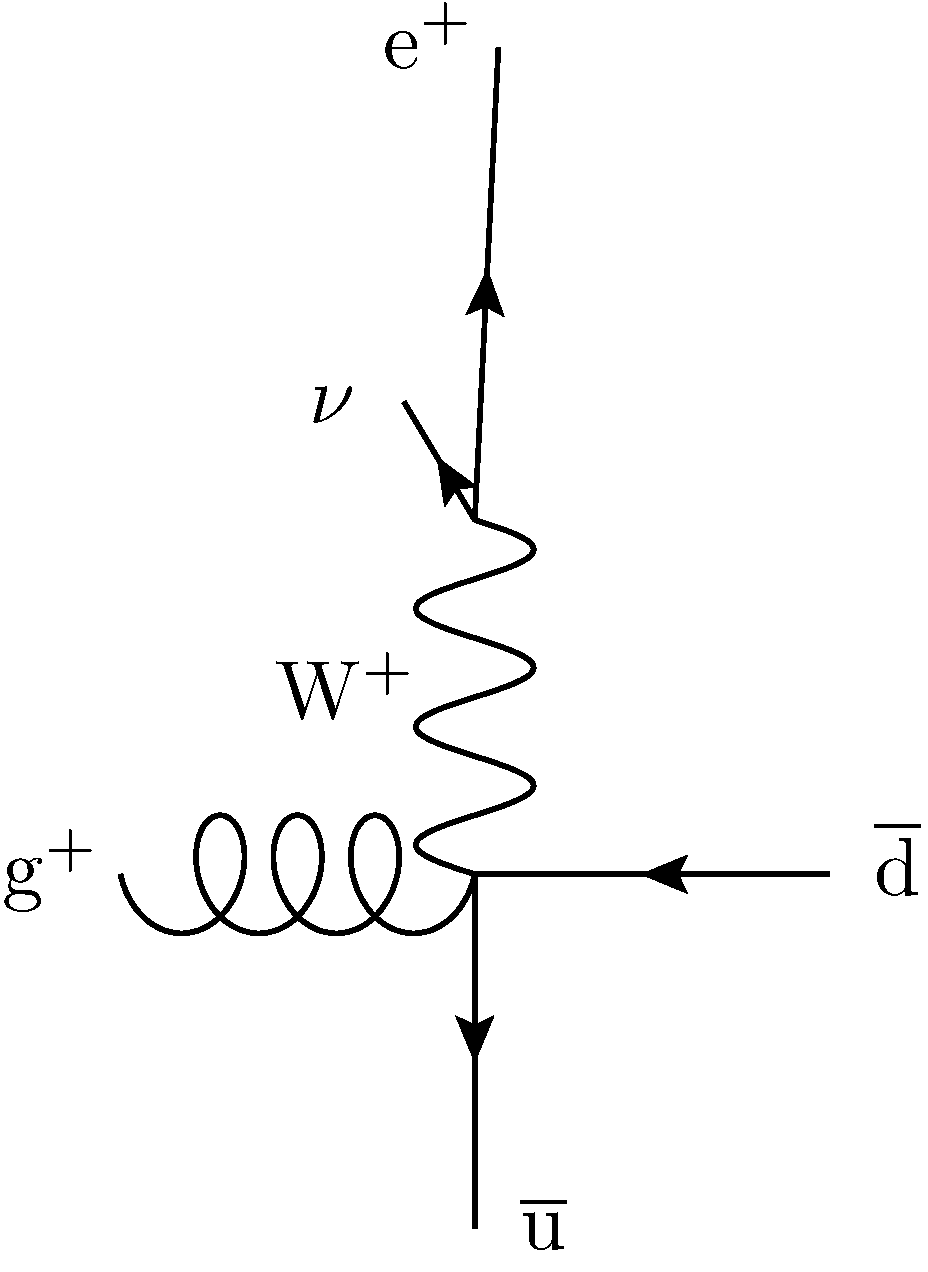
\includegraphics[width=0.3\textwidth]{fig/wpol_prod_f}}
\caption{Illustrations of $\PWplus+1$~jet production modes at the LHC. The
  $\Pgluon$ superscript indicates its helicity}
\label{fig:w1jet_modes}
\end{figure}
  \chapter{Searching for Supersymmetry in the Single Lepton Channel at CMS}
  \chapter{Interpretation of Search Results Within Theoretical Models}
\section{Introduction}
It is very often the case that a search for \ac{NP} will yield results
consistent with the currently accepted theory (which, in most particle physics
contexts would be the \ac{SM}). In the absence of a discovery\footnote{Certain
  models may also have a role to play in the characterisation of a discovery.},
it is often desirable to provide additional information in the form of a
statistical interpretation of the results. Such an interpretation typically
serves the following goals:
\begin{itemize}
\item Indicate the strength of the analysis in searching for the proposed model
  or set of models. This can then be used as an objective measure by which to
  rank different analyses or to benchmark the progress of a single analysis as
  data is collected.
\item Falsify, to some confidence level, a particular theory or some region of
  parameter space within that theory. In the case of a reasonably generic model,
  parameterised in such a way that it may represent other theories (or
  approximate their experimental signature), theorists may be able to
  test the predictions of a variety of models directly against the results of
  the interpretation. This will be discussed further in Section~\ref{sec:sms}.
\item Guide the optimisation of analysis cuts and object selection.
\end{itemize}

Providing an interpretation invariably necessitates some choice of theory or
phenomenological model against which to test the results. The range of theories
will of course depend strongly on the inclusiveness of the experiment. Indeed,
in many cases a single theory will have motivated the analysis in the first
place and the choice of model will be clear. In other cases, the analysis have
been designed to be as inclusive as possible and therefore sensitive to an array
of theories. Typically this is achieved by focussing on a particular detector
signature (for instance missing transverse energy), where a deviation from the
\ac{SM} is a common feature of many \ac{NP} scenarios. Another similar issue
arises when the model being tested is not well defined with a large number of
free parameters which affect the experimental expectations.

\ac{SUSY} searches in particular are subject to these
considerationss. Firstly, as discussed in Section~\ref{sec:susy}, the theory
has a large number of free parameters which may drastically change the
experimental signature. Secondly, whilst a \ac{SUSY} specific interpretation is
possible in principal, it is in some sense not the best use of the experimental
data. The large, multi-dimensional \ac{SUSY} parameter space and corresponding
variation in the physics signatures necessitates an inclusive analysis
strategy - typically looking for high jet multiplicities in association with
large missing transverse energy. Such signatures may occur in a variety of
potential \ac{NP} theories. With an appropriate interpretation, the results of
an inclusive \ac{SUSY} search can be used to draw conclusions about these
theories, restricting their parameter space or ruling them out altogether.

\ac{SUSY} searches at the \ac{LHC} have typically provided two
interpretations. The first, within a very restricted class of \ac{SUSY} theories
known as the \ac{CMSSM}. The second, within one or more so-called ``Simplified
Models'', chosen by theorists to represent a wide range of possible \ac{NP}
theories, categorised according to their phenomenological properties.

\section{Models}
\subsection{\acl{CMSSM}}

\subsection{Simplified Models}
\label{sec:sms}
It is often the case that theorists, having devised some theory, and made
concrete phenomenological predictions from it, wish to test it against
experimental data. The difficulty then arises of taking these predictions and
translating them into a form where they can be compared directly with
experimental results. Typically, these results will be provided in the form of
one or more event yields, corresponding background predictions and statistical
and systematic uncertainties. In some (but probably not most) cases, the
relevant correlations will also be included. The theorist must then take the
predictions of the theory and apply experimental resolution effects to them in
order to simulate the expected signal yield. Modern detectors are highly complex
and require very complex simulation to precisely model all of the resolution
and acceptance effects. In some cases, in particular for relatively simple
kinematic quantities, a simplified parameterisation may suffice but detailed
checks will be required to confirm that a given approximation reproduces, with
adequate fidelity the full detector simulation or the actual recorded data. If
it can be confirmed that this is the case, the theorist may then proceed to redo
the work of the experimentalist in modelling the various statistical and
systematic effects in the form of a likelihood function. Finally, they may then
utilise all of these components to produce their own statistical interpretation
of the data against the chosen theory.

Clearly, this procedure is both laborious and error-prone. It was therefore
proposed that the \ac{LHC} experiments would provide a richer interpretation in
the context of a set of ``Simplified Models''. Broadly speaking, a simplified
model is a highly simplifed effective theory, chosen to characterise a
particular phenomological scenario present within one or more \ac{NP}
models. Free parameters which have little effect on the physics are integrated
out, leaving only those with a large effect on the physics. In constructing a
number of these models, the full space of possibly physical signatures arising
in much more complicated theories may be spanned.

Although the concept of a simplified model is quite general, the discussion here
will focus on those inspired by \ac{SUSY} or ``\ac{SUSY}-like'' theories, and
more specifically those relevant to the single-leptonic experimental search
described in previous chapters.

% \todo[size=\tiny, linespacing=0.5]{Mention that SMS are used for characterisation of discovery as well as
%   design of searches}

\subsubsection{Dark Matter Models}
As discussed in Chapter~\ref{sec:susy}, a highly desirable prediction of certain
supersymmetric theories is the existence of a stable, weakly-interacting
particle or \ac{WIMP}. This is a dark matter candidate with a striking
experimental signature at collider experiments - a large missing energy
component in the transverse plane. At hadron colliders, the initally produced
particles are likely to be coloured (either squarks or gluinos) which will then
decay to the \ac{WIMP} producing a large number of jets. Together, these might
be considered the characteristics of a ``canonical'' \ac{SUSY} event at the
\ac{LHC}. Whilst the range of simplified models includes a much more generic set
of signatures, for the purposes of this discussion we will choose two topologies
which exhibit these characteristics.

Both topologies emulate certain aspects of \ac{SUSY} phenomenology albet in a
simpler framework with greater generality. In order to distinguish the particle
content from pure \ac{SUSY} theories, a different notation will be used. The
first topology, T1 arises from pair production of neutral, coloured objects
$\tilde{G}$ (the gluinos of \ac{SUSY} theories). The second topology, T2 instead
arises from pair production of a charged, coloured particle $\tilde{Q}$
(effectively the squark). Both topologies consider only pair-produced
superpartners or in other words they conserve an $R$-parity type quantum
number. In addition to the superpartners produced in the intial interaction,
there are a number of intermediate states $\tilde{X}^0_i$ and
$\tilde{X}^{\pm}_j$. In terms of \ac{SUSY} particles these would be analogues of
the neutralinos and charginos respectively. Importantly, $\tilde{X}^0_1$ is defined to
be the lightest superpartner - a dark matter candidate and the source of missing
energy in the events.

\subsubsection{T1 Simplified Model Topology}
In the T1 simplified model, the $\tilde{Q}$ are assumed to be heavier than the
$\tilde{G}$ and thus the only decay mode available is via an off-shell
$\tilde{Q}$. Three such cascade decays leading to the $\tilde{X}^0_1$ are shown in
Figure~\ref{fig:gluino_sms_decays}. The first, is a direct 3-body decay to the
\ac{LSP}. This dominates in the following \ac{mSUGRA} scenarios:
\begin{itemize}
\item $\PSgxzi \approx \PSB$ and the $\PSq_{R}$ are lightest or the $\PSW$ is kinematically
  inaccessible.
\item $\PSgxzi \approx \PSW$ and either $\PSq_{L}$ are lightest or there is no
  splitting between the left and right-handed squarks.
\item $\PSgxzi \approx \PSH$ and either heavy-flavour squarks are inaccessible or
  $\PSB$ and $PSW$ are inaccessible.
\end{itemize}

\begin{figure}
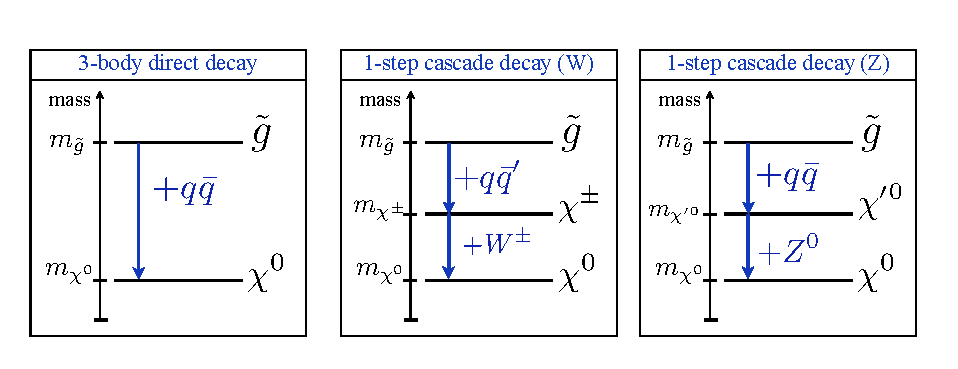
\includegraphics[width=\textwidth]{fig/gluino_sms_decays}
\caption{Illustration of the gluino decay modes within the T1 simplified model
  topology. \cite{alves_simplified_2011}}
\label{fig:gluino_sms_decays}
\end{figure}

In most \ac{mSUGRA} or \ac{GMSB} models, the $\PSgxzi \approx \PSB$ and there is
not a strong left-right mass splitting in the squarks. Therefore, it is unlikely
for the direct decays to dominate. In most cases, 1-step cascade decays
will be favoured. In these the, gluino decays first to either a $\PSgxpm$ or a
heavy $\PSgxz$. This will subsequently decay via either a $\PW$ or a $\PZ$ to
the $\PSgxzi$.

\subsubsection{T2 Simplified Model Topology}
For the T2 simplified model, the produced $\tilde{Q}$ can decay as follows:
\begin{eqnarray}
\tilde{Q} &\longrightarrow \tilde{G} \Pq \label{eqn:t2gluino}\\
\tilde{Q} &\longrightarrow \tilde{X}^0_i \Pq \\
\tilde{Q} &\longrightarrow \tilde{X}^\pm_i \Pq
\end{eqnarray}
If allowed, the \ref{eqn:t2gluino} decay will dominate since it has QCD
strength.

\subsubsection{Combining Topologies}
For phenomenological purposes, each separate decay topology may be considered as
an independent simplified model. The predictions of a whole set of topologies
can then be combined by taking linear combinations. For direct comparison
against experimental data, it is desirable to simulate a desired set of
topologies within a monte-carlo generator by ``turning on'' the chosen physics
subprocesses. The model parameter space can be sampled by moving through a
lattice of values in the desired range. At each lattice site, a statistically
sufficient number of events is generated with the appropriate parameter values
inserted into the configuration of the \ac{MC} generator.

\section{Statistical Methods}
\subsection{Background}

\subsection{Modelling the Single Lepton Analysis}
As described in the previous section, the core component of many statistical
interpretations is the construction of an appopriate likelihood function. The
likelihood must model all statistical and systematic effects and is thus highly
dependent on the experiment. The situation is considerably complicated when
shape information is included, for which relevant bin-to-bin correlations must
be included.

\subsubsection{Notation}
It will be helpful to define some notation. In the following, a subscript index
is assumed to run over the binned variable in the analysis
(i.e. \STlep). All nuisance parameters are written as $\nu^{(i)}$ where the
superscript index is taken to run over some set of systematics
(e.g. $\nu^{\textrm{jes}}$ might represent a jet energy scale
uncertainty). Certain variables $x$ are known to have a functional dependence on a
given nuisance parameter and are written $x(\nu)$. The nominal value of this
variable, being that which is measured in \ac{MC} or in real data is denoted
$\bar{x}$.

\subsubsection{The Likelihood Function}
In constructing the likelihood, we start by writing down the number of events
expected for each bin (assigned the index $i=0,1,2...$):
\begin{equation}
\NExpi = \NSigi(\mu, \nu^{(j)}) +
\NBkgi(\nu^{(k)}) \\
\end{equation}
where \NSigi is the expected signal yield for a chosen
signal model and \NBkgi is the data-driven background
prediction. As can be seen, the signal yield is a function of the \ac{poi} (the
signal strength) and some number of nuisance parameters where the index $j$
will run over a set of systematics relevant to the signal yield. Ignoring
signal contamination effects (which will be discussed later), the bacground
yield depends only on the nuisance parameters $\nu^{(k)}$ where $k$ is taken to run
over the set of systematics relevant to the bacground prediction.

Without giving an explicit functional form for the signal yield and background
prediction, the form of the likelihood function may be constructed. The
likelihood must include:
\begin{enumerate}
\item Statistical terms representing the likelihood of observing the given
  number of events given a certain expectation for the signal and background
  yields.
\item Terms providing prior constraints on the various nuisance
  parameters. Certain uncertainties are statistical in nature and thus,
  indepdent nuisance parameters are assigned per bin along with a corresponding
  prior pdf. In other cases, the underlying systematic variation is considered
  to have a 100\% correlated effect across the bins. In these cases, a single
  nuisance parameter and prior pdf is assigned.
\end{enumerate}

The form of the likelihood is as follows,
\begin{equation}
\mathcal{L} = \prod_i \Poisson(\NExpi ; \NObsi)
\prod_{\alpha \in \Theta}  X_\alpha(\nu^{(\alpha)})
\end{equation}
where
\begin{itemize}
\item $\mathcal{P}(\mu;x)$ denotes a Poisson distribution with mean $\mu$ and value
$x$
\item The $X_\alpha(\nu^{(\alpha)})$ represent some prior pdf associated with
  each systematic $\alpha$.
\end{itemize}

\subsubsection{The Signal Yield}
The signal yield per bin is constructed as follows
\begin{equation}
\NSigi = \mu \times \epsilon_i(\nu^{(\alpha)}) \times \sigma \times L \times \nu^{\textrm{lumi}}
\end{equation}

with
\begin{itemize}
\item $\epsilon_i(\nu^{(\alpha)})$ is the efficiency of the $i$th bin assumed to be
  dependent on a set of nuisance parameters $\nu^{(\alpha)}$.
\item $\sigma$ the cross-section of the signal model being considered,
\item $L$ the integrated luminosity,
\item $\nu^{\textrm{lumi}}$ the nuisance parameter associated with uncertainty in the
estimate of the integrated luminosity.
\end{itemize}

\subsubsection{Background Prediction}
The background prediction per bin is then written as
\begin{equation}
\NBkgi = \RCSi(\nu_i^{(\alpha)}, \nu^{(\beta)}) \times \NControli(\nu_i^{(\gamma)})
\end{equation}
where
\begin{itemize}
\item \RCSi is the translation ratio as defined in Section TODO,
\item The nuisance parameters $\nu_i^{(\alpha)}$ and $\nu_i^{\gamma}$ represent
  statistical uncertainties uncorrelated between the bins.
\item The nuisance parameters $\nu_i^{(\beta)}$ represent systematic
  uncertainties assumed to be 100\% correlated across the bins.
\item \NControli the observed number of events in the control region
($L_P > 0.3$)
\end{itemize}

\subsubsection{Parameterising Systematics}
In reality, it is almost always impossible to obtain a full functional form for
a variable $x$ (e.g. \RCSi, \NControli) in terms of a set of nuisance parameters
$\nu^{(\alpha)}$. Writing the Taylor expansion of $x(\nu^{(\alpha)})$ for two terms to
second order,
\begin{align*}
 x(\nu^{(A)}, \nu^{(B)})\bigg|_{\substack{\nu^{(A)} = a\\ \nu^{(B)} = b}} \approx
x(a,b) +
(\nu^{(A)} - a)\left.\frac{\partial x}{\partial\nu^{(A)}}\right|_{\nu^{(A)}=a} +
(\nu^{(B)} - b)\left.\frac{\partial x}{\partial\nu^{(B)}}\right|_{\nu^{(B)}=b} +\\
\frac{1}{2!}\left[
(\nu^{(A)} - a)^2 \frac{\partial^2 x}{\partial \left(\nu^{(A)}\right)^2}
+ (\nu^{(B)} - b)^2 \frac{\partial^2 x}{\partial \left(\nu^{(B)}\right)^2}
+ 2(\nu^{(A)} - a)(\nu^{(B)} - b)\frac{\partial^2 x}{\partial
  \nu^{(A)}\partial\nu^{(B)}}
\right]
\end{align*}
Assuming the expansion is performed with respect to the mean of x, $\bar{x}$,
the values of $a$ and $b$ are seen to be the mean values of the corresponding nuisance
parameters. For small deviations from the mean,
\begin{equation}
 (\nu^{(A)} - a) \sim (\nu^{(B)} - b) \sim \epsilon \sim 0
\end{equation}
and ignoring terms $O(\epsilon^2)$

\begin{equation}
x(\nu^{(A)}, \nu^{(B)}) \approx \bar{x} +
(\nu^{(A)} - a)\left.\frac{\partial x}{\partial\nu^{(A)}}\right|_{\nu^{(A)}=a} +
(\nu^{(B)} - b)\left.\frac{\partial x}{\partial\nu^{(B)}}\right|_{\nu^{(B)}=b}
\label{eqn:stats:taylor}
\end{equation}
Since the derivatives in Equation~\ref{eqn:stats:taylor} will in practice be
derived from some finite variation of the underlying quantity associated with
each nuisance parameter, the infinitessimal derivatives must be replaced by
finite changes. It is also sensible to set $a=b=0$.
\begin{equation}
x(\nu^{(A)}, \nu^{(B)}) \approx \bar{x} +
\nu^{(A)}\frac{\Delta x}{\Delta\nu^{(A)}} +
\nu^{(B)}\frac{\Delta x}{\Delta\nu^{(B)}}
\label{eqn:stats:taylor2}
\end{equation}
Since the value of $x$ is often associated with a physical quantity such as an
efficiency or an event yield, it is desirable to constrain it to positive
values. This can be achieved providing the range of each nuisance parameter is
set such that
\begin{equation}
\nu^{(\alpha)}\times\frac{\Delta x}{\Delta \nu^{(\alpha)}} < \bar{x}
\end{equation}

The previous derivation can be simply extended two $N > 2$ nuisance
parameters. Generalising and rewriting Equation~\ref{eqn:stats:taylor2},
\begin{eqnarray*}
x(\nu^{(A)}, \nu^{(B)}, \ldots) &\approx& \bar{x} +
\nu^{(A)}\frac{\Delta x}{\Delta\nu^{(A)}} +
\nu^{(B)}\frac{\Delta x}{\Delta\nu^{(B)}} + \ldots \\
&\approx& \frac{1}{\bar{x}^{N-1}} \left\{ \bar{x}^N +
\bar{x}^{N-1} \nu^{(A)}\frac{\Delta x}{\Delta\nu^{(A)}} +
\bar{x}^{N-1} \nu^{(B)}\frac{\Delta x}{\Delta\nu^{(B)}} + \ldots \right\}
\end{eqnarray*}
Trying to rewrite as a product,
\begin{eqnarray*}
\prod_{j=A, B, \ldots} \left(\bar{x} + \frac{\Delta x}{\Delta\nu^{(\alpha)}}\right) &=&
\bar{x}^N + \bar{x}^{N-1} \sum_{j=A, B, \ldots} \nu^{(\alpha)}\frac{\Delta x}{\Delta \nu^{(\alpha)}} \\
&&+ \bar{x}^{N-2}\sum_{j=A, B, \ldots} \sum_{k=A, B, \ldots} \nu^{(\alpha)}\nu^{(\beta)}\frac{\Delta x}{\Delta
  \nu^{(\alpha)}}\frac{\Delta x}{\Delta \nu^{(\beta)}} \\
&&+ \ldots +O(\nu^N)
\end{eqnarray*}
Ignoring terms greater than $O(\nu^2)$,
\begin{eqnarray*}
\prod_{j=A, B, \ldots} \left(\bar{x} + \frac{\Delta x}{\Delta\nu^{(\alpha)}}\right) &\approx&
\bar{x}^N + \bar{x}^{N-1} \sum_{j=A, B, \ldots} \nu^{(\alpha)}\frac{\Delta x}{\Delta
  \nu^{(\alpha)}} \\
&\approx& \bar{x}^{N-1} x(\nu^{(A)}, \nu^{(B)}, \ldots)
\end{eqnarray*}
and therefore
\begin{equation}
x(\nu^{(A)}, \nu^{(B)}, \ldots) \approx \frac{1}{\bar{x}^{N-1}} \prod_{j = A, B,
  \ldots} \left(\bar{x} + \frac{\Delta x}{\Delta\nu^{(\alpha)}}\right) \approx
\bar{x} \prod_{j = A, B,
  \ldots} \frac{1}{\bar{x}}\left(\bar{x} + \frac{\Delta x}{\Delta\nu^{(\alpha)}}\right)
\label{eqn:stats:systderiv}
\end{equation}

Using Equation~\ref{eqn:stats:systderiv}, the signal yield can be rewritten as follows
\begin{equation}
\NSigi = \mu \times \bar{\epsilon}_i \times \prod_{j}\left(\frac{\bar{\epsilon}_i
    + \nu^{(\alpha)}\frac{\Delta\epsilon_i}{\Delta\nu^{(\alpha)}}}{\bar{\epsilon}_i}\right) \sigma \times L \times \nu^{\textrm{lumi}}
\end{equation}
and the background prediction
\begin{equation}
\NBkgi = \RbarCS_i \times \prod_{j}\left( \frac{\RbarCS_i
    + \nu^{(\alpha)}\frac{\Delta\RCSi}{\Delta\nu^{(\alpha)}}}{\RbarCS_i}\right)
\times \NbarControl_i \times \prod_{k}\left( \frac{\NbarControl_i
    + \nu^{(\alpha)}\frac{\Delta\NControli}{\Delta\nu^{(\beta)}}}{\NbarControl_i}\right)
\end{equation}

\subsection{Nuisance Parameters}
The nuisance parameters incorporated in the model described thus far are of two
types.
\begin{enumerate}
\item Statistical uncertainties assumed to be uncorrelated across analysis
  bins. This includes uncertainties arising from limited generator statistics,
  limited data in the control region and signal contamination in the control
  region.
\item Systematic uncertainties arising from detector artefacts or theoretical
  uncertainties such as jet energy scale, standard model cross-sections and
  integrated luminosity measurement.
\end{enumerate}
For uncertainties of the first kind, independent nuisance paramters must be
included for each analysis bin. For uncertainties of the second kind, a
single nuisance parameter will be included for all bins. This achieves the
desired correlation. A full list of the nuisance parameters used is shown in
Table~\ref{tbl:systematic_parameters}.

\ctable[
cap=Nuisance parameters included in the single lepton likelihood function,
caption=Summary of nuisance parameters included in the single lepton likelihood function.,
mincapwidth=0.5\textwidth,
label=tbl:inter_systematic_parameters,
pos=h,
doinside=\scriptsize
]{lccccc}{
\tnote[a]{Muon channel only}
\tnote[b]{Electron channel only}

\tnote[c]{In the electron channel, the use of \ac{MC} templates in the QCD
  background estimate introduces a dependence on the \ac{JES}. Whilst the
  ability to include these correlations was added to the statistics package, it
  was not used in the results shown.}

}{\FL
Uncertainty                        & Correlated & \NSigi     & \RCSi      & \NControli & Nuisance Parameters\ML
%
Luminosity                         & \checkmark & \checkmark &            &            & $\nu^{\textrm{lumi}}$\NN
\acf{JES}                          & \checkmark & \checkmark & \checkmark & \tmark[c]  & $\nu^{\textrm{jes}}$\NN
\MET Resolution                    & \checkmark & \checkmark & \checkmark & \tmark[c]  & $\nu^{\textrm{metres}}$\NN
\PW/\Ptop\APtop Ratio              & \checkmark &            & \checkmark &            & $\nu^{W\Ptop\APtop}$\NN
\PW Polarisation                   & \checkmark &            & \checkmark &            & $\nu^{\textrm{\PW pol}}$\NN
Muon Momentum Scale\tmark[a]       & \checkmark &            & \checkmark &            & $\nu^{\textrm{lep}}$\NN
Limited \ac{MC} Statistics         &            &            & \checkmark &            & $\nu^{\textrm{MC}}_i$\NN
Limited Data Statistics            &            &            &            & \checkmark & $\nu^{\textrm{data}}_i$\NN
Signal Contamination               &            &            &            & \checkmark & $\nu^{\textrm{sig cont}}_i$\NN
\ac{PDF} Uncertainties             & \checkmark & \checkmark &            &            & $\nu^{\textrm{pdf}}_i$\NN
QCD Background Prediction\tmark[b] &            &            &            & \checkmark & $\nu^{\textrm{qcd}}_i$\LL
}

\subsection{Signal Contamination}
It can be seen in Figure~TODO that the region \LPcontrol may have a substantial
component of \ac{SUSY} events depending on the particular model under
consideration. Signal contamination increases \NControl leading to an
overprediction of \NBkg. To account for this, the \NBkgi term is modifed to
reflect the assumption that some fraction of the yield in \NControli will be
due to \ac{SUSY} contamination. Rewriting,

\begin{equation}
\NBkgi(\mu, \nu^{(\alpha)}) = \RbarCS_i \times \prod_{j}\left( \frac{\RbarCS_i
    + \nu^{(\alpha)}\frac{\Delta\RCSi}{\Delta\nu^{(\alpha)}}}{\RbarCS_i}\right)
\times \NbarControl_i \times f^{\textrm{SM}}_i(\mu) \times \prod_{k}\left( \frac{\NbarControl_i
    +
    \nu^{(\alpha)}\frac{\Delta\NControli}{\Delta\nu^{(\beta)}}}{\NbarControl_i}\right)
\end{equation}
where $f^{\textrm{SM}}_i$ represents the fraction of \NControli expected to be
\ac{SM} events given the signal hypothesis. The prior distribution assigned to
this systematic in \likelihood is then
\begin{equation}
X(\nu^{\textrm{SM}}) = \Gauss \left( \frac{\NControli}{\NControli + \mu\times\epsilon_i^{\textrm{control}}\times\sigma\times L}
; \nu^{\textrm{SM}} \right)
\end{equation}
and $f^{\textrm{SM}}_i = \nu^{\textrm{SM}}_i$. Due to technical difficulties with
introducing these terms into the likelihood, it was rewritten as follows
\begin{equation}
X(\nu^{\textrm{SM}}_i) = \Gauss \left( \frac{\NControli}{\NControli + \epsilon_i^{\textrm{control}}\times\sigma\times L}
; \nu^{\textrm{SM}}_i \right)
\end{equation}
and the term included in the background prediction becomes
\begin{equation}
f^{\textrm{SM}}_i = 1 - \mu \times \left(1- \nu^{\textrm{SM}}_i\right)
\end{equation}
This can be justified as follows
\begin{eqnarray}
<f^{\textrm{SM}}> &=& 1 - \mu \times \left(1-<\nu^{\textrm{SM}}>\right) \\
                  &=& 1 - \mu  + \mu\times\frac{\NControli}{\NControli + \NSUSYi} \\
                  &=& \frac{(1-\mu)\left(\NControli + \NSUSYi\right) + \mu\NControli}{\NControli + \NSUSYi} \\
                  &=& \frac{\NControli + (1 - \mu)\NSUSYi}{\NControli + \NSUSYi} \\
                  &=& \frac{\NControli \left( 1 + (1-\mu)\frac{\NSUSYi}{\NControli}\right)}{\NControli + \NSUSYi} \\
                  &=& \frac{\NControli}{\left(\NControli +\NSUSYi\right)\left( 1 + (1 - \mu)\frac{\NSUSYi}{\NControli}\right)^{-1}} \\
                  &\approx& \frac{\NControli}{\left(\NControli +\NSUSYi\right)\left( 1 - (1-\mu)\frac{\NSUSYi}{\NControli}\right)} \\
                  &=& \frac{\NControli}{\NControli + \mu\NSUSYi - (1-\mu)\frac{\NSUSYi^2}{\NControli}}
\end{eqnarray}



\section{Results}

\begin{figure}
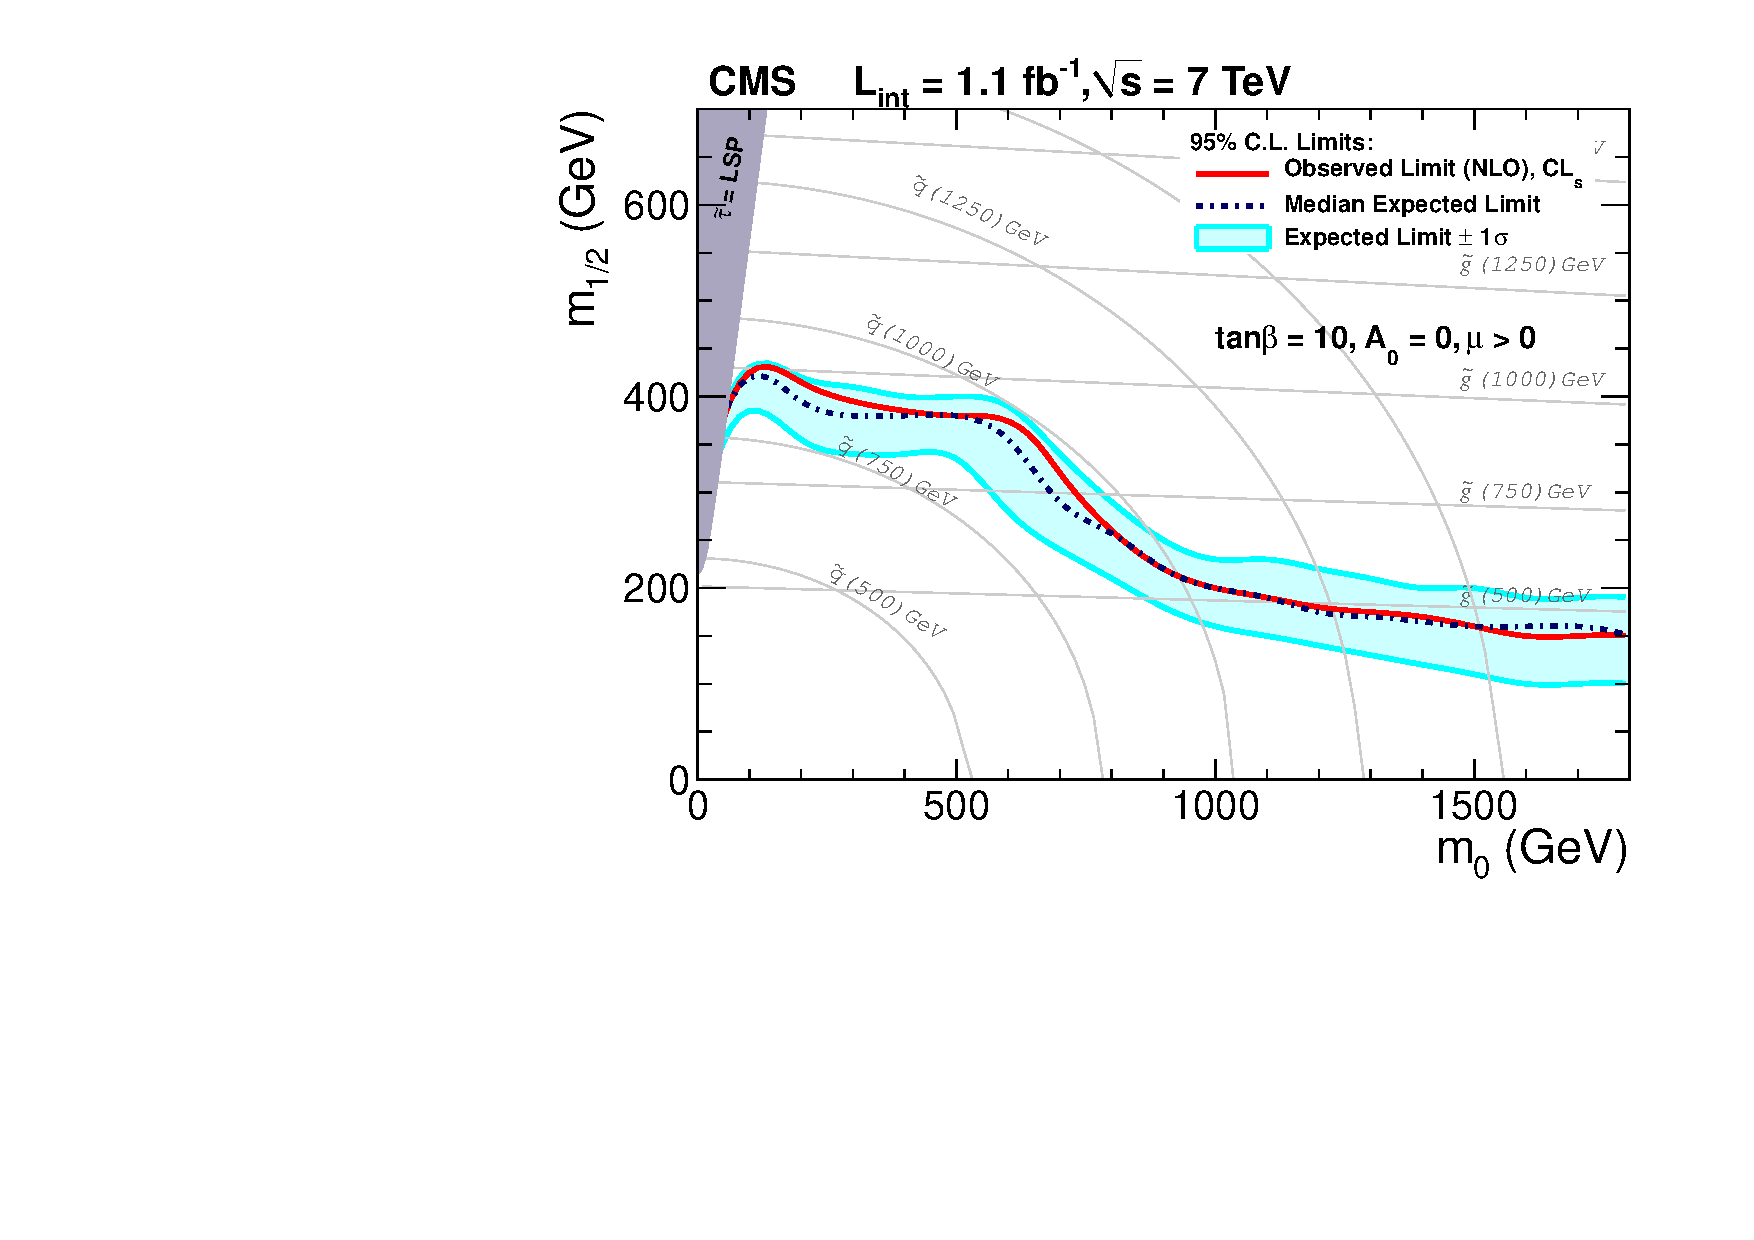
\includegraphics[width=\textwidth]{fig/RA4_ExclusionLimit_tanb10}
\end{figure}
%%% Local Variables:
%%% mode: latex
%%% TeX-master: "../thesis"
%%% End:

\end{comment}

%% Produce the appendices
\begin{appendices}
  
\chapter{Kinematics}
A Lorentz tranformation can be written as
\begin{equation}
\left(\begin{array}{c} E' \\ p_{\parallel}' \end{array} \right)
=
\left(
\begin{array}{cc}
\gamma & -\gamma\beta \\
-\gamma\beta & \gamma
\end{array}
\right)
\left (\begin{array}{c} E \\ p_{\parallel} \end{array}\right)
\end{equation}
and
\begin{equation}
p_{\perp}' = p_{\perp}
\end{equation}

Boosting from a particles rest frame into the lab frame,
\begin{equation}
\left(\begin{array}{c} E \\ P \end{array} \right)
=
\left(
\begin{array}{cc}
\gamma & -\gamma\beta \\
-\gamma\beta & \gamma
\end{array}
\right)
\left (\begin{array}{c} M \\ 0 \end{array}\right)
\end{equation}
and so
\begin{eqnarray*}
E &=& \gamma M  \Longrightarrow \gamma = \frac{E}{M} \\
|P| &=& \gamma\beta M \Longrightarrow \beta = \frac{|P|}{\gamma M} = \frac{|P|}{E}
\end{eqnarray*}
also
\begin{eqnarray*}
\gamma &=& \frac{\sqrt{P + M}}{M} \\
&=& \sqrt{1 +\left(\frac{|P|}{M}\right)^2}
\end{eqnarray*}

\end{appendices}

%% Produce the un-numbered back matter (e.g. colophon,
%% bibliography, tables of figures etc., index...)
\begin{backmatter}
  \bibliographystyle{lucas_unsrt}
\bibliography{shorttitles,bibstrings,thesis}

\begin{colophon}
  A number of software tools were vital to the production of this thesis. The
  author is extremely grateful to the many individiuals responsible. Without
  such high-quality tools, this work would simply not have been possible.

The thesis was written using the \textsc{Emacs} text-editor and typeset with
\TeX/\LaTeX using the \textsc{HEPThesis} package. The \texttt{git} version
control system was invaluable for maintaining backups and managing changes.

All work was performed using the \textsc{GNU/Linux} operating system, primarily
the variant assembled by the volunteers of the \textsc{Arch Linux} project. Much
of the code was written using the \textsc{Python} programming language. Whilst
some plots were produced using the \textsc{ROOT} framework, the author
recommends \texttt{matplotlib} for its superior API and powerful features.
\end{colophon}

\end{backmatter}

%% Close
\end{document}

;; %%% Local Variables:
;; %%% TeX-command-default: "SCons"
;; %%% mode: latex
;; %%% TeX-PDF-mode: t
;; %%% TeX-master: "thesis"
;; %%% End:
